\subsection{Normalizing constant estimation}
\label{subsec:estim_constant}
In order to illustrate the \IFIS\, estimator, motivate the choice of the dissipative Hamiltonian dynamics, and test the different parameters at stake, consider first the problem of estimating the normalizing constant of a mixture of Gaussian distributions in dimension $d$. The target distribution here is 
\[
p: y \mapsto5\left\{\Normal(y;-\mathbf{u}_d, \sigma^2 I_d) +  \Normal(y;\mathbf{u}_d, \sigma^2 I_d)\right\}\eqsp,
\]
where $\Normal(\cdot,\mu,\Omega)$ is the Gaussian probability density function with mean $\mu$ and variance $\Omega$, $\mathbf{u}_d$ is the $d$ dimensional vector with all coordinates set to 1 and $\sigma^2 = 0.02$. We choose a flat proposal distribution $\rho$ defined as a $d$-dimensional centered Gaussian, with diagonal covariance $\sigma^2_\rho I_d$, $\sigma^2_\rho=10$. %We choose $d=10$ in our experiments. %Consider a flat proposal distribution $\rho$, which is assumed to cover the different modes of the target distribution. 
The performance of the $\IFIS$ estimator is first illustrated in this toy problem for $d=10$ and different choices of parameters, using the test function $p/\rho$. 

Our approach is compared to a naive importance sampling scheme which samples points from  $\rho$. %, which is assumed to cover the different modes of the target distribution.%, and would compute the estimator $\hat{Z}_n = 1/n \sum_{k\leq n} p(X^i)/\rho(X^i)$, where $x^i\sim \rho$.
The $\IFIS$ estimator is also compared to a  tuned AIS estimator \cite{neal:2001}, a state-of-the-art competitor for the estimation of normalizing constants.
AIS builds on a series of MCMC kernels to build an efficient importance distribution. Typically, the MCMC kernels use Langevin or Hamiltonian dynamics, which makes it directly comparable to our estimator.

We present four examples of trajectories with different values for the damping factor $\gamma$. The performance of the associated estimators are displayed in \Cref{fig:simple_gauss}. %The target distribution here is a mixture of 2 $d$-dimensional concentrated Gaussians (diagonal covariance $\sigma^2 = 0.02$ ), 
%\[
%p(z) = \tfrac{1}{2}(\Normal(y;-\mathbf{u}_d, \sigma^2\Id) +  \Normal(y;\mathbf{u}_d, \sigma^2\Id))\eqsp,
%\]
%where $\mathbf{u}_d$ is the $d$ dimensional vector with all coordinates set to 1. 
%We choose $\rho$ to be a $d$-dimensional centered Gaussian, with diagonal covariance $\sigma^2_\rho \Id$, $\sigma^2_\rho=10$. We choose $d=10$ in our experiments. 
All estimators are run 100 times with a similar computational budget, and we report the mean and standard deviation for each method. Figure~\ref{} displays a boxplot for each estimator.
We use $n = 20000$ samples for $\IFIS$ estimator and AIS, with a trajectory and an annealing schedule of length $K=10$ in both cases, to match computational budget. The stepsize is set to $h= 0.1$ for both the Hamiltonian transformation of $\IFIS$ estimator and the leapfrog steps of AIS. 
Finally, the Importance Sampling estimator uses $K\times n$ samples for a fair comparison in terms of computational budget. Section~\ref{} provides additional experiments in more challenging settings to illustrate how the $\IFIS$ algorithm is an appealing solution to estimate normalizing constants.
\begin{figure}
    \centering
    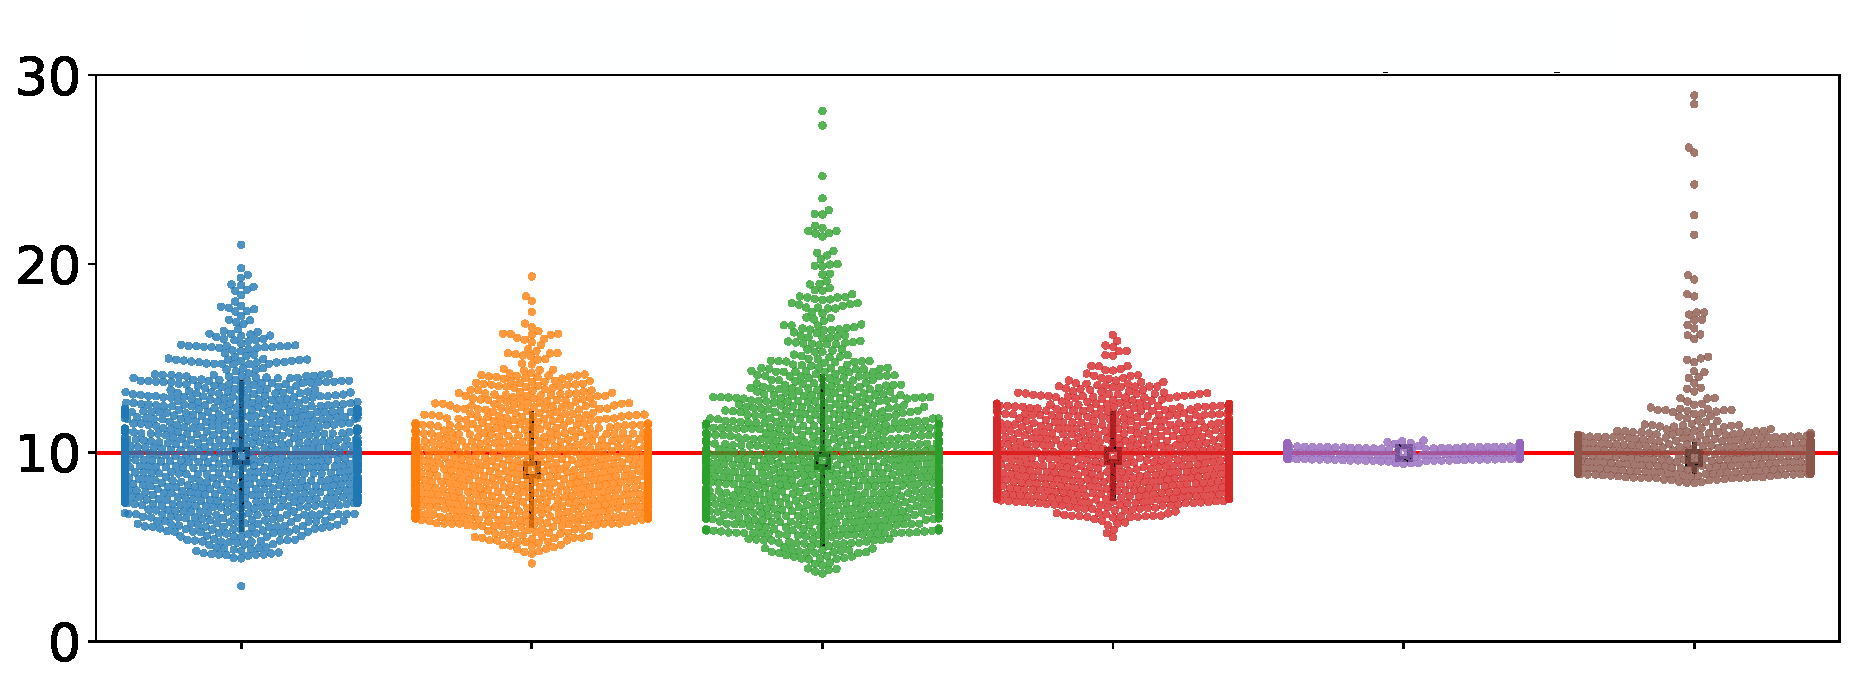
\includegraphics[width= \linewidth]{pics/boxplot_two_gaussian_dim_5.pdf}
    \caption{Results for the estimation of the normalizing constant in the toy example:  a mixture of two peaked Gaussians, in dimension 5. The true value is $Z=10$ (red line)}
    \label{fig:simple_gauss}
\end{figure}
\begin{comment}
\begin{table}[]
\caption{Results for the estimation of the normalizing constant in the toy example:  a mixture of two peaked Gaussians, in dimension 5. The true value is $Z=1$.}
\label{tab:simple_gaussian_est}
\begin{tabular}{c|c|c|}
\cline{2-3}
                                                 & Mean & Standard deviation \\ \hline
\multicolumn{1}{|c|}{IS estimate}                &    $6\cdot10^{-5}$  &           $6\cdot10^{-4}$         \\ \hline
\multicolumn{1}{|l|}{AIS estimate}               &  $3\cdot10^{-3}$    &    $2\cdot10^{-2}$                \\ \hline
\multicolumn{1}{|l|}{$\IFIS$ - $\gamma=0$}   &   $0.49$   &      4.9              \\ \hline
\multicolumn{1}{|l|}{$\IFIS$ - $\gamma=1$} &  $0.45$    &          2.5          \\ \hline
\multicolumn{1}{|l|}{$\IFIS$ - $\gamma=3$}   &   0.93   &   0.31                 \\ \hline
\multicolumn{1}{|l|}{$\IFIS$ - $\gamma=6$}   &  1.0    &        0.64            \\ \hline
\end{tabular}
\end{table}
\end{comment}
